\documentclass[12pt]{article}

\usepackage[utf8]{inputenc}
\usepackage{geometry}
\geometry{a4paper,scale=0.75}
\linespread{1.5}
\usepackage{graphicx} 
\usepackage{float} 
\usepackage{subcaption} 
\usepackage{enumerate}
\usepackage{enumitem}
\usepackage{amsmath}
\usepackage{array}
\usepackage{booktabs}
\usepackage{multirow}
\usepackage{amsfonts}
\usepackage[english]{babel}
\usepackage{amsthm}
\usepackage{dcolumn}
\usepackage{multicol}
\usepackage{stfloats}
\usepackage{lscape}
\usepackage[figuresright]{rotating}
\RequirePackage{pdflscape}
\usepackage[toc,page]{appendix}
\usepackage{geometry}
\usepackage{longtable}
\usepackage{comment}
\usepackage{xcolor}

% -------- enumerated sub-labels (a), (b), … --
\usepackage{enumitem}
\setlist[enumerate,1]{label=(\alph*),ref=\alph*}
% ---------------------------------------------

\usepackage{hyperref}
\hypersetup{hidelinks,
	colorlinks=true,
	allcolors=black,
	pdfstartview=Fit,
	breaklinks=true}
\usepackage{csquotes}
\usepackage{natbib}
\bibliographystyle{apalike}
\newtheorem{definition}{Definition}
\newtheorem{theorem}{Theorem}
\newtheorem{proposition}[theorem]{Proposition}
\newtheorem{lemma}[theorem]{Lemma}
\newtheorem{corollary}[theorem]{Corollary}
\newtheorem*{remark}{Remark}
\newtheorem{example}{Example}
\newtheorem{exercise}{Exercise}
\newtheorem{assumption}{Assumption}[section] % number within sections


\begin{document}

\begin{center}
    ECON 3123: Macroeconomic Theory I\\
    {\large \textbf{Tutorial Note 8: IS-LM-PC Framework}}\\
    Teaching Assistant: Harlly Zhou
\end{center}

\subsection*{Deriving the PC Relation}
To put IS-LM and PC together, we need either interest rate or output appear in the PC relation. By this, we mean that we would like to derive a step further from the Phillips curve so that, obviously easier to show, output appears.

Recall that the production function is
\[Y_t = A N_t,\]
where $Y_t$ is the output, $A$ is the productivity, and $N_t$ is the labour force, and that unemployment rate $u_t$ is defined to be
\[u_t = \frac{L-N_t}{L},\]
where $L$ is total labour force minus discouraged worker.
Hence,
\[u_t = 1-\frac{1}{A}\frac{Y_t}{L} \iff Y_t = AL(1-u_t).\]
We can thus define \textbf{the natural level of employment}, $N_n$, and \textbf{the natural level of output}, $Y_n$:
\[N_n = L(1-u_n),\,\, Y_n = AL(1-u_n),\]
where $u_n$ is the natural rate of unemployment.

Then we can rewrite the Phillips Curve equation to obtain the \textbf{PC relation}:
\begin{align*}
    \pi_t - \pi_t^e &= -\alpha (u_t - u_n)\\
    &= -\alpha\left[\left(1-\frac{1}{A}\frac{Y_t}{L}\right) - \left(1-\frac{1}{A}\frac{Y_n}{L}\right)\right]\\
    &= \frac{\alpha}{AL}(Y_t - Y_n).
\end{align*}

Figure \ref{fig:pc01} demonstrates how a PC curve looks like in a $(Y, \pi-\pi^e)$ diagram. From the mathematical formulation, we know that the line must pass $(Y_n,0)$. This is supported by economics: when the market is in medium-run equilibrium, inflation expectation matches the true inflation, and the output is at the natural level. Let $\pi^e=\bar{\pi}$, the targeted inflation. Then in this diagram, the corresponding output $Y_t$ is larger than the natural level. In this case $N_t > N_n$, and $u_t < u_n$.
\begin{figure}[htp]
    \centering
    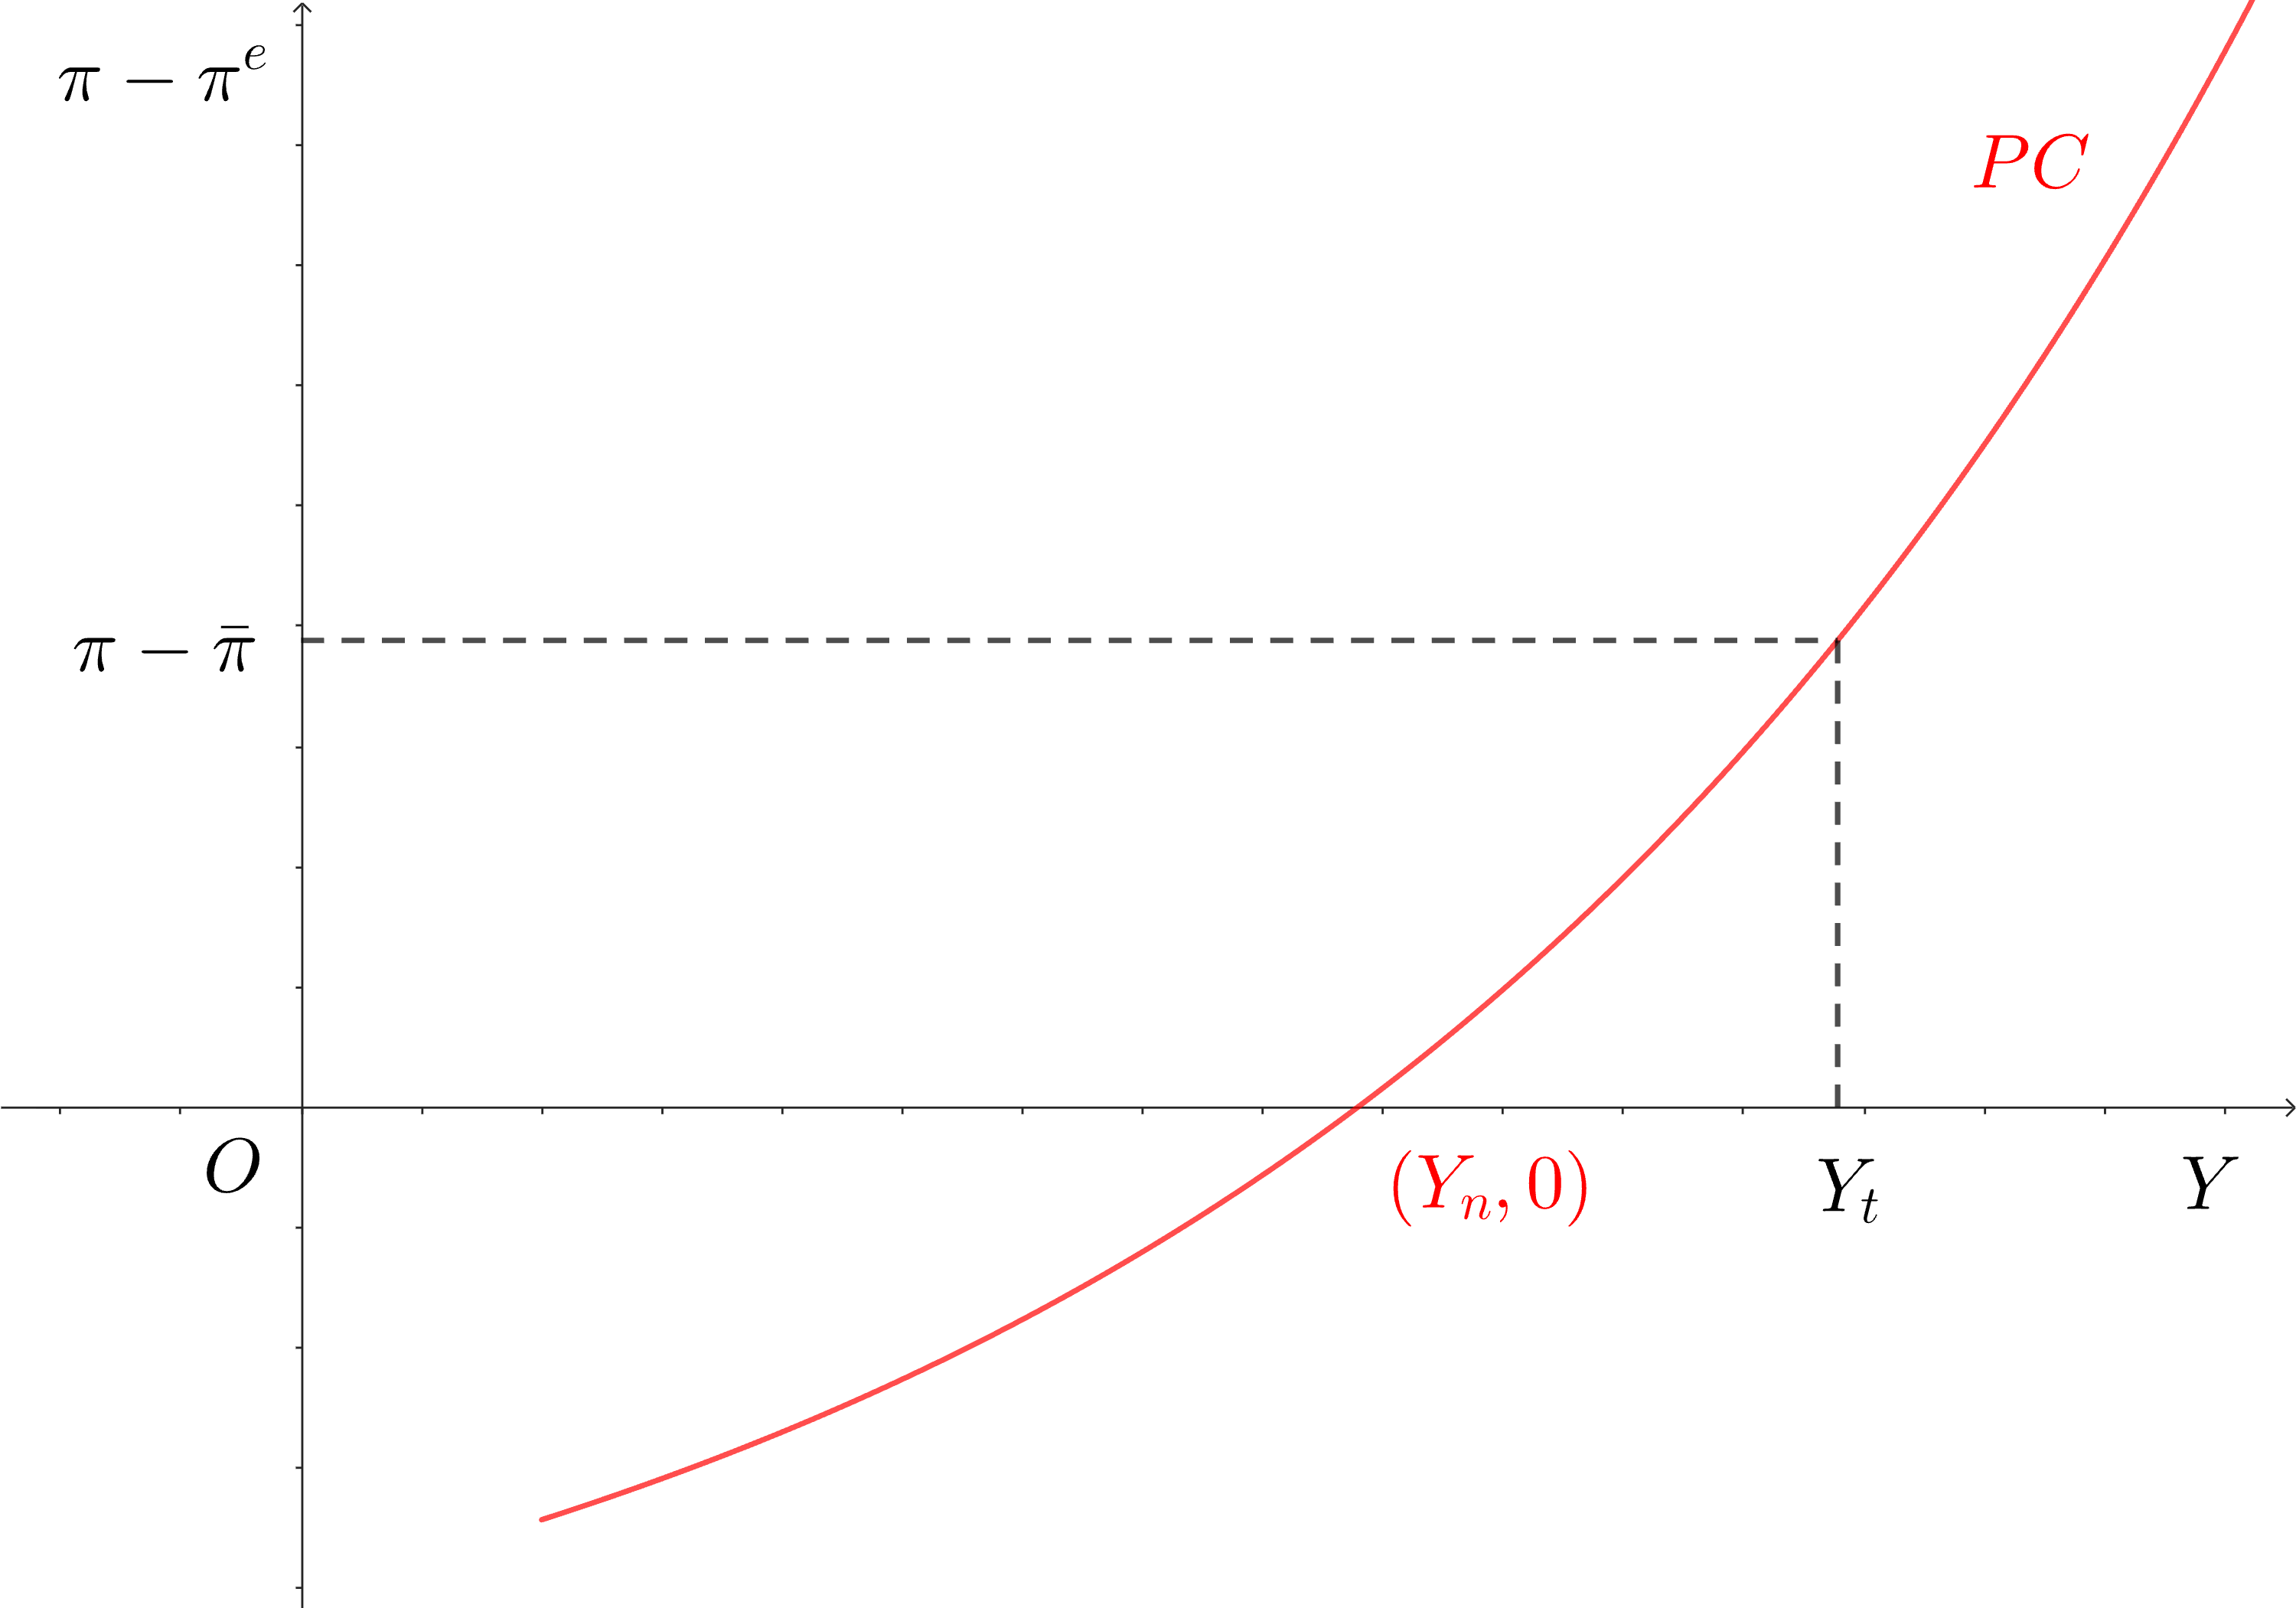
\includegraphics[width=0.6\textwidth]{pc01.png}
    \caption{PC Relation}
    \label{fig:pc01}
\end{figure}

\subsection*{Neutrality of Money}
With the medium run framework to be introduced, we are able to find the role of money in an economy. In short, in the medium run, real variables are \textit{not} affected by the monetary policy (money supply), but only the inflation and nominal interest rate. 

\paragraph{IS-LM-PC Framework}
The IS-LM framework is one for short run, and the labour market will be at the equilibrium in the medium run. Therefore, the key point is to make out how the economy changes in the process from short run to the long run.

The following figure \ref{fig:is-lm-pc} illustrates how the equilibrium moves from the short run to the medium run. Initially, in the short run ($IS$-$LM$), we have equilibrium $(Y^*, r)$. Assume that the central bank does not change the interest rate. Then the labour market ($PC$) indicates that the inflation is higher than the targeted rate. Therefore, the central bank will, at some point, adjusts the monetary policy (say, cutting money supply) so that the real interest rate increases. It will reach a point where the equilibrium output in the $IS$-$LM$ diagram matches the natural level of output derived in the labour market equilibrium. The corresponding real interest rate is thus called the \textbf{natural/neutral/Wicksellian rate of interest}.

  \begin{figure}[htbp]
    \centering
    \begin{subfigure}[t]{0.6\textwidth}
      \centering
      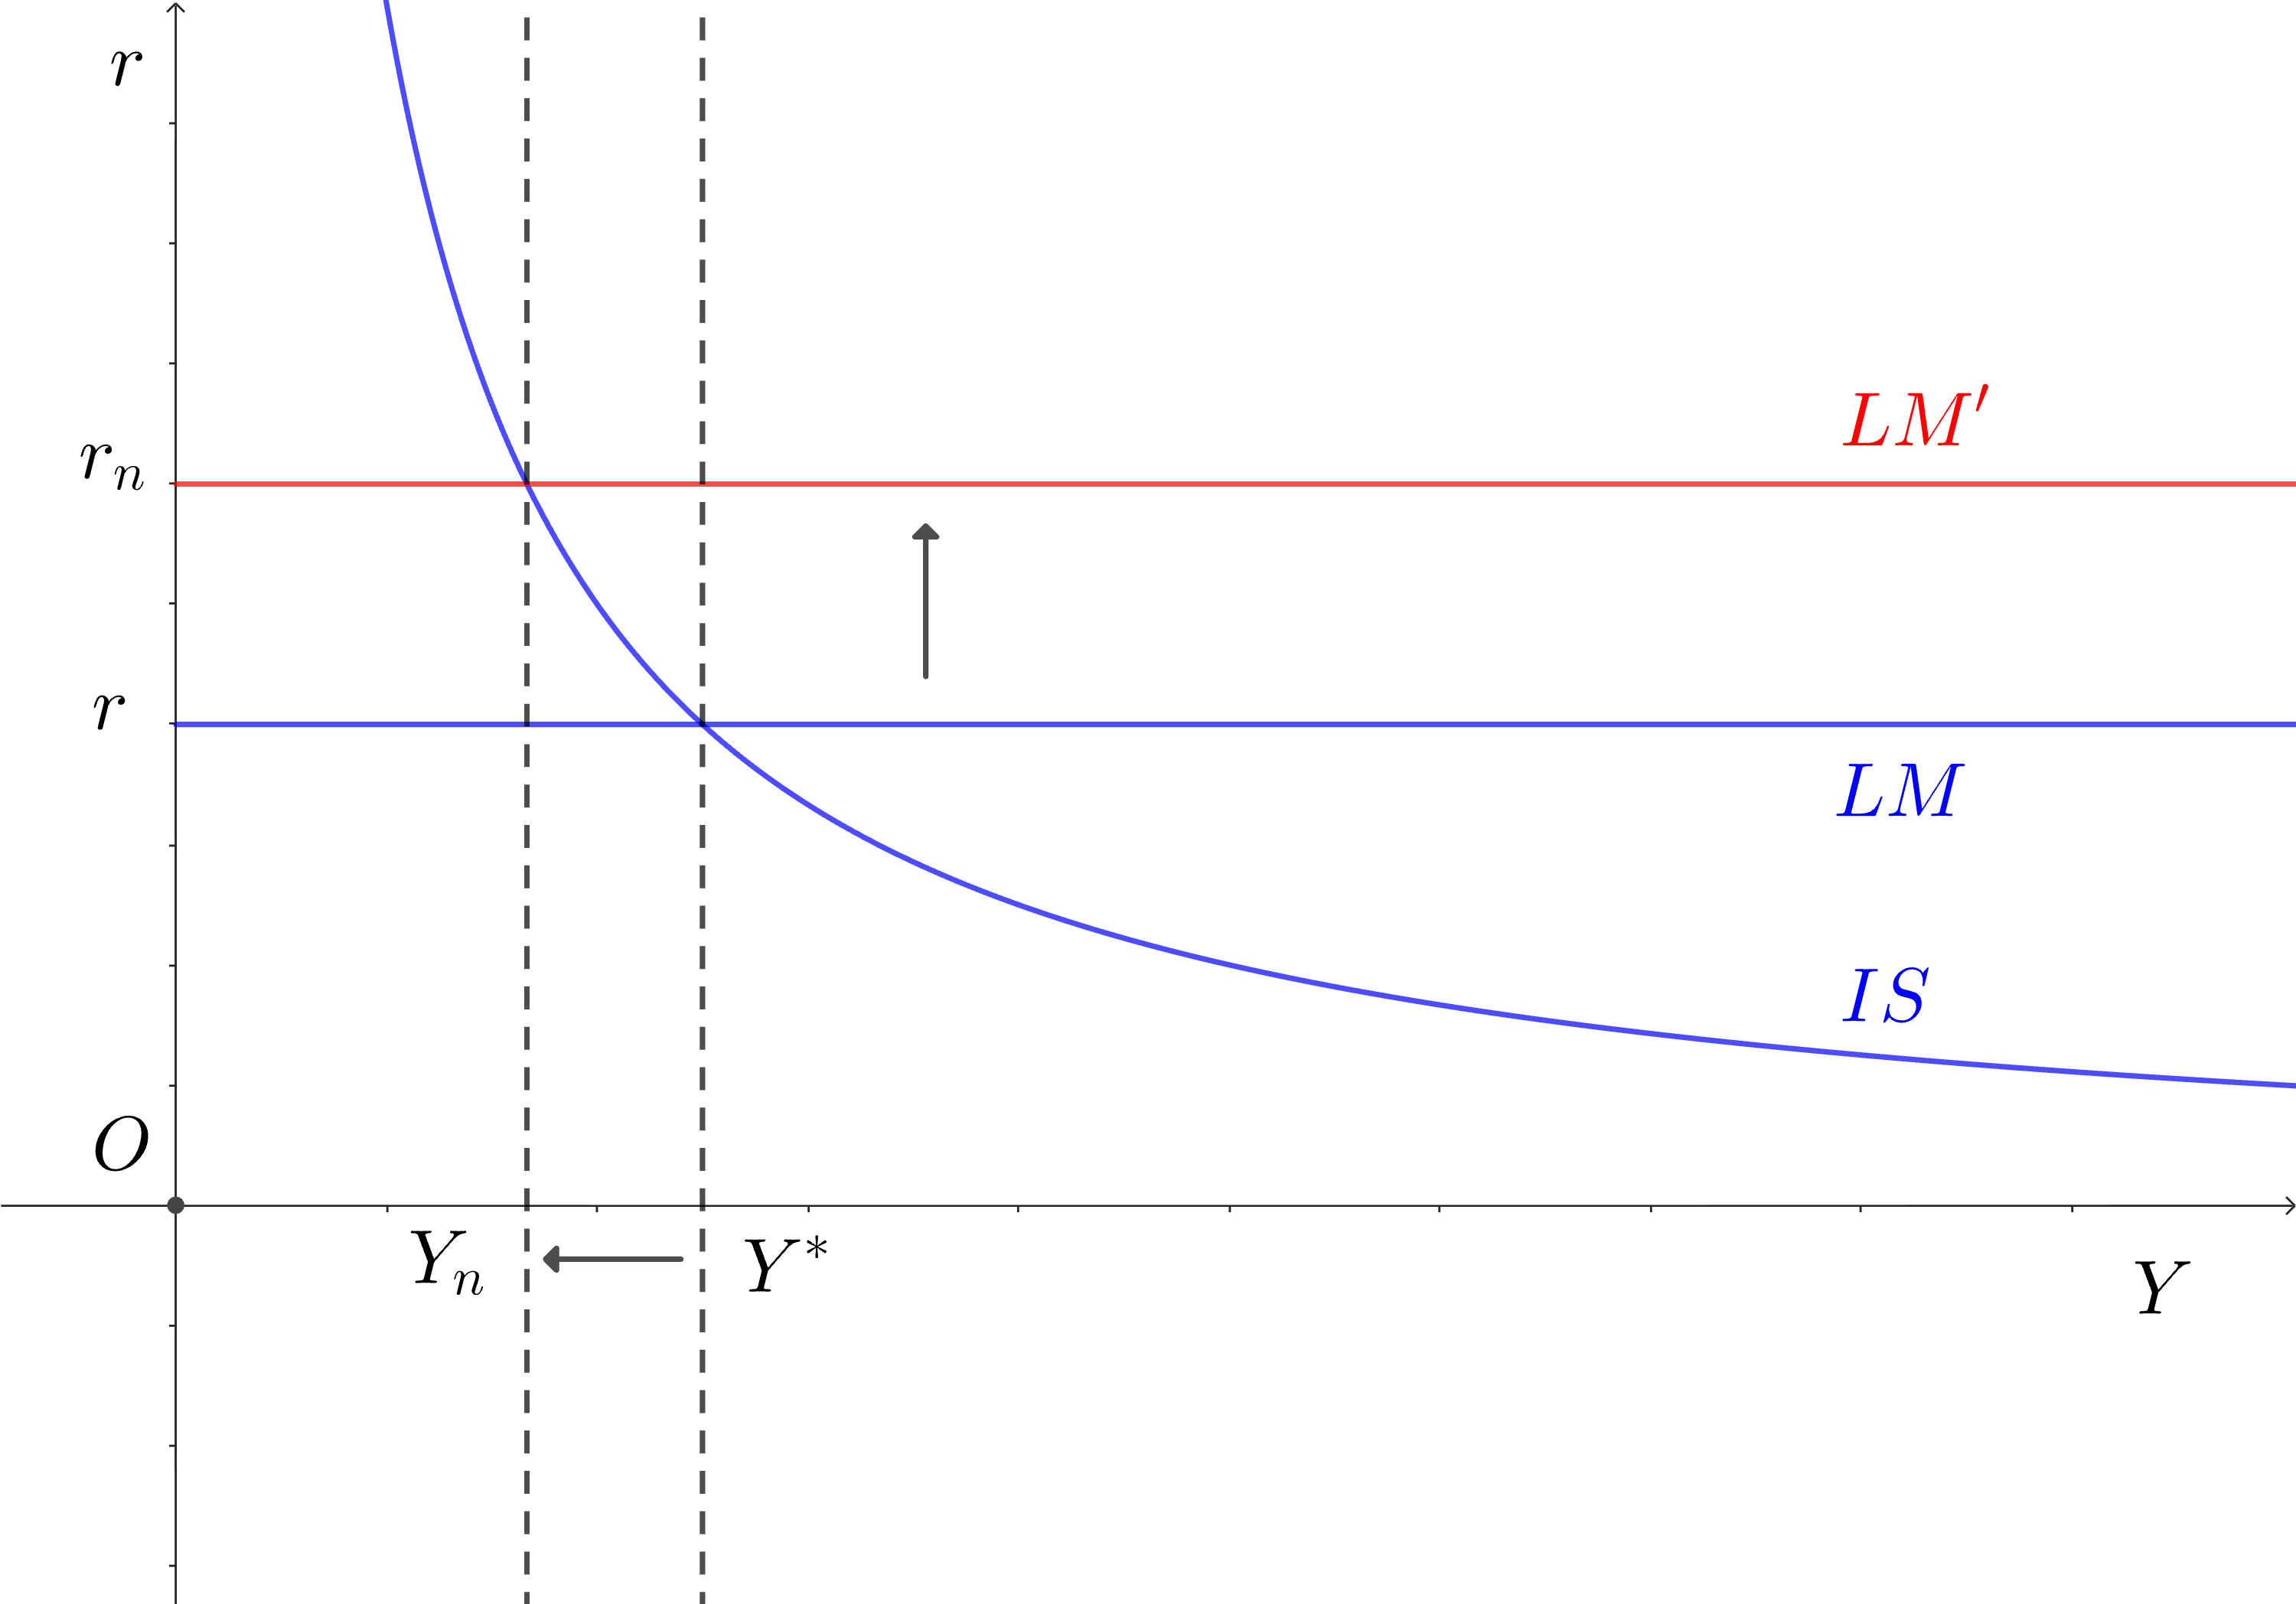
\includegraphics[width=\linewidth]{islmpc01.png}
    \end{subfigure}\hfill
    \begin{subfigure}[t]{0.6\textwidth}
      \centering
      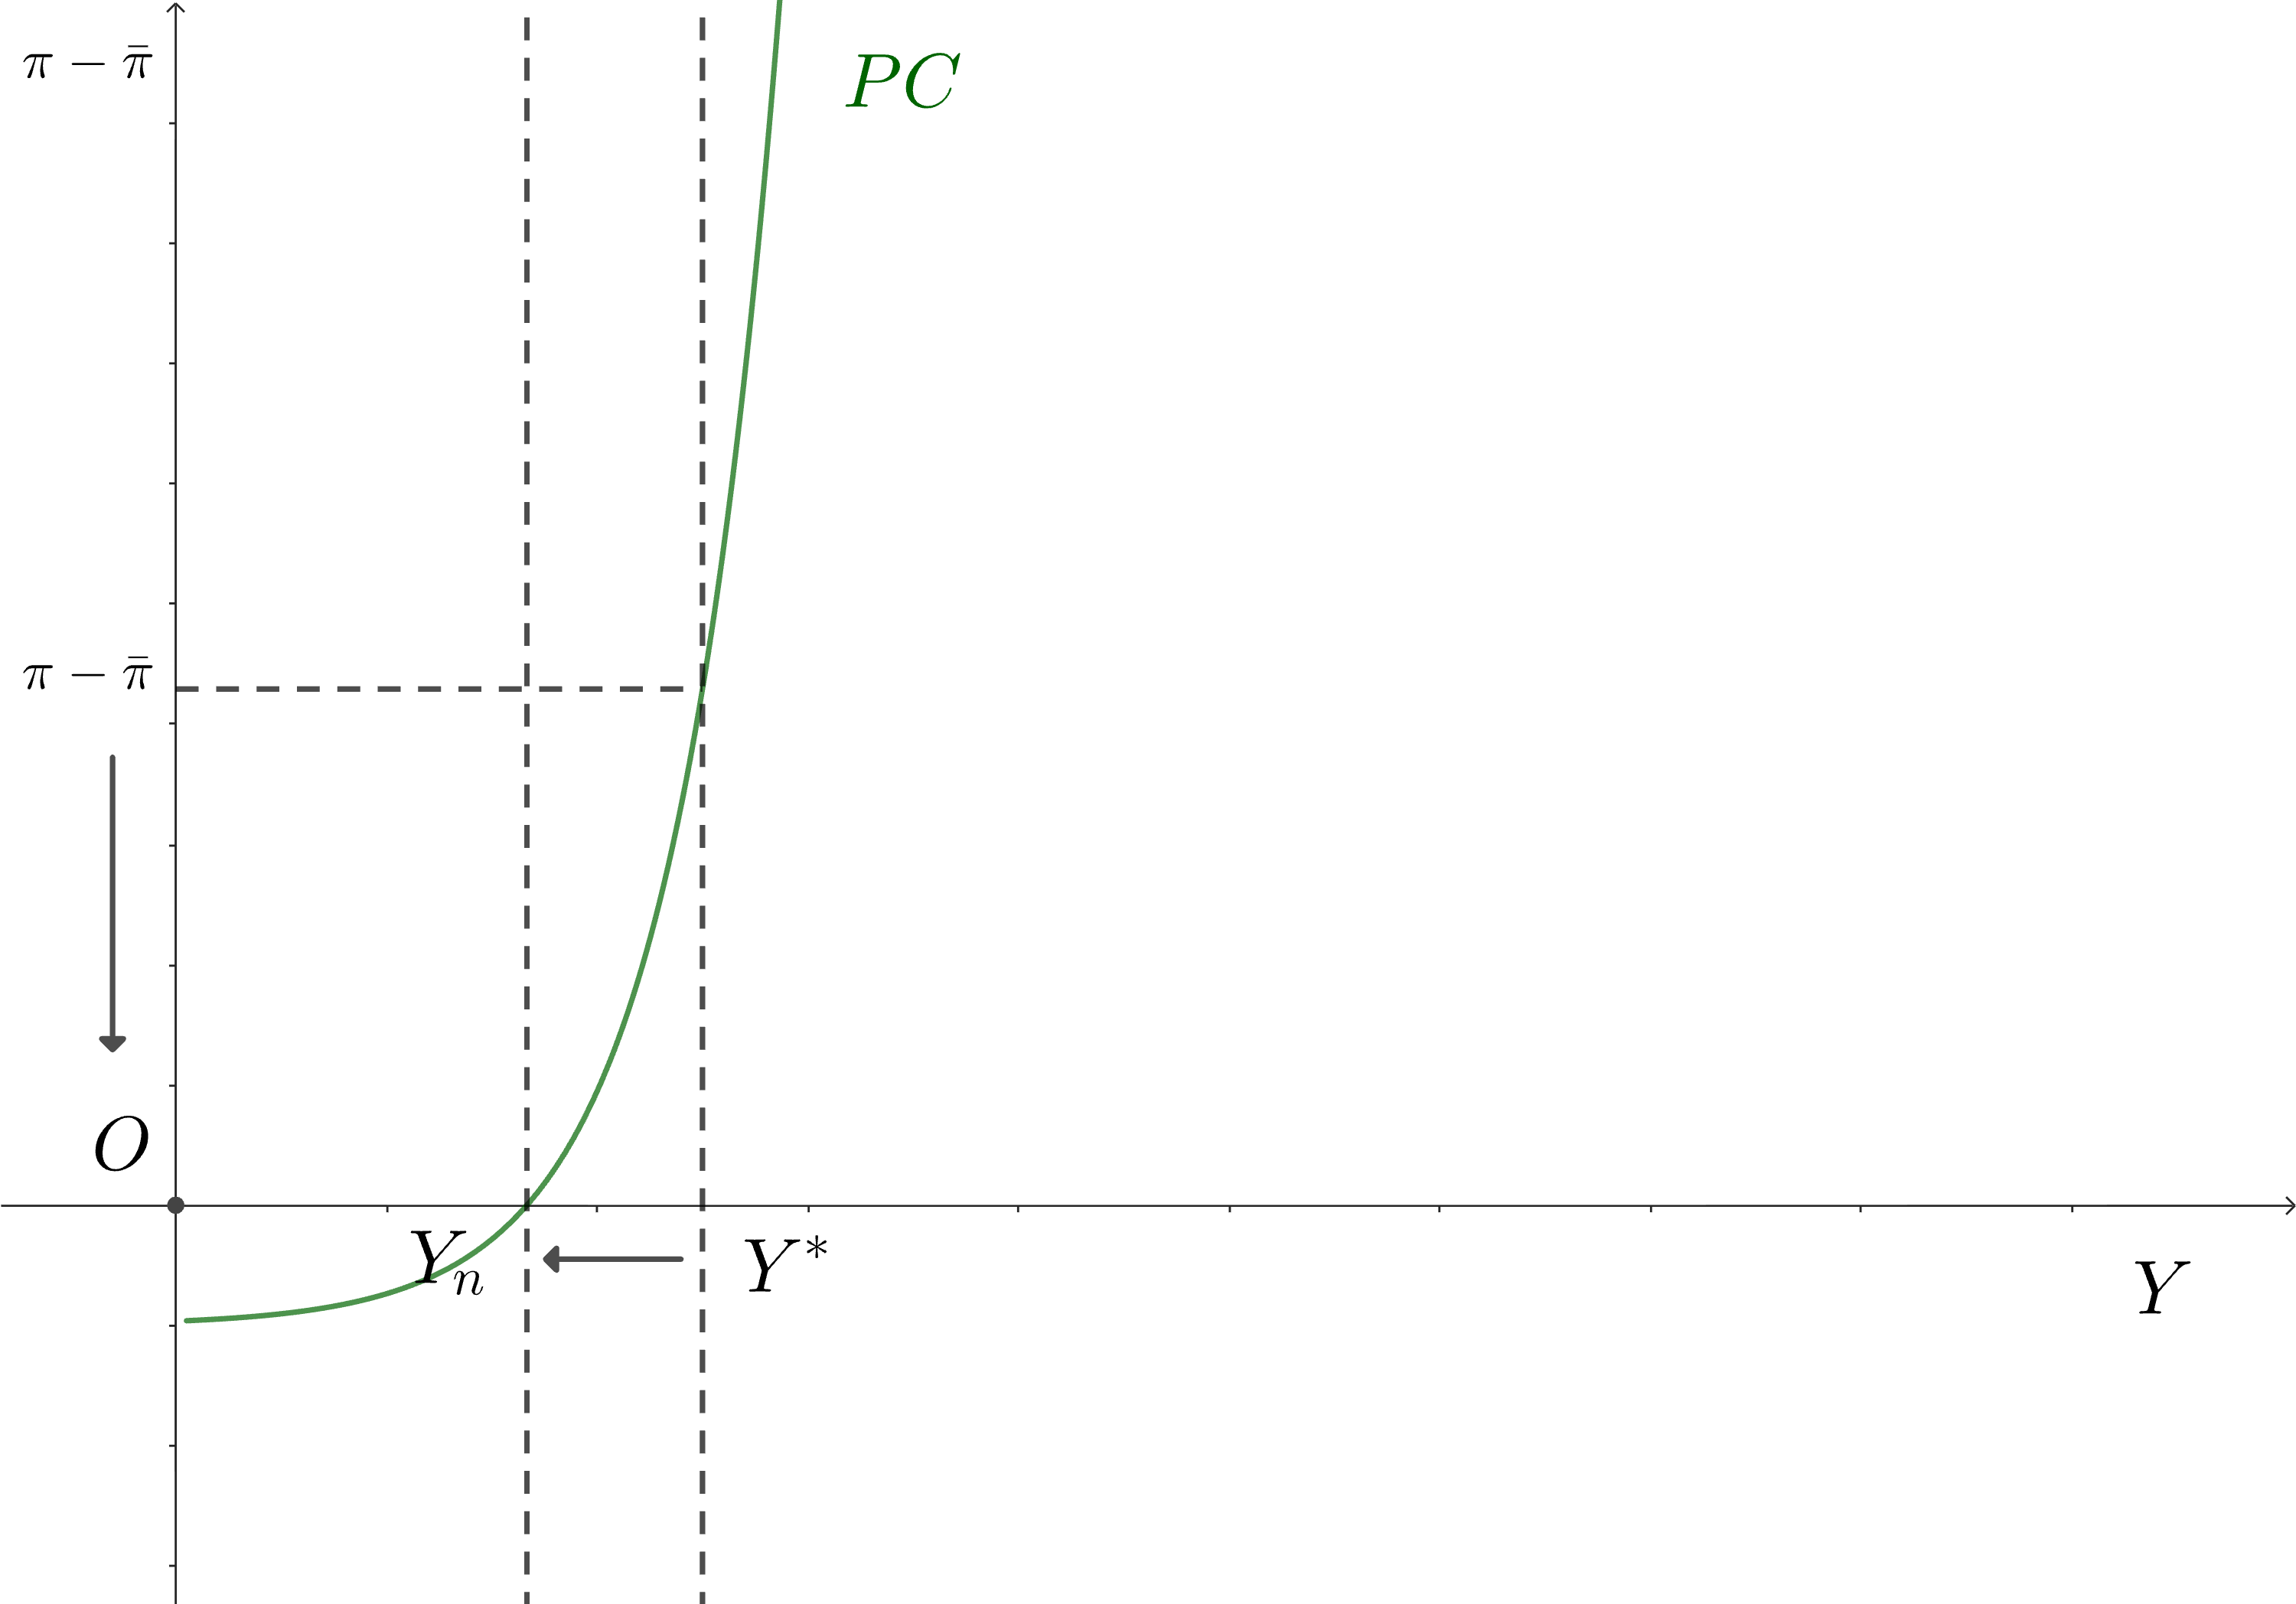
\includegraphics[width=\linewidth]{islmpc02.png}
    \end{subfigure}
    \caption{IS-LM-PC Framework}
    \label{fig:is-lm-pc}
  \end{figure}

\paragraph{Money Market Equilibrium}
Recall that the money demand function is
\[\frac{M^d_t}{P_t} = Y_t \mathcal{L}(r_t+\pi^e_{t+1})\]
where $\mathcal{L}$ is a decreasing function of $i_t = r_t + \pi^e_{t+1}$.
At medium-run equilibrium,
\begin{align*}
    M &= M^d = M^s,\\
    Y &= Y_n,\\
    r &= r_n, \text{and }\\
    \pi&= \pi^e = \bar{\pi}.
\end{align*}
Therefore, the equilibrium money supply is
\[\frac{M}{P} = Y_n \mathcal{L}(r_n + \bar{\pi}).\]
Note that the RHS is just a constant. Hence, the real equilibrium money supply is a number. Therefore, money and price must grow at the same rate, \textit{i.e.},
\[\pi = g_M.\]
Then we know that any monetary policy (changing money supply) can only affect the inflation, and thus the nominal interest rate in the medium run. Real variables are not affected. This is called the \textbf{neutrality of money}. In PhD Macroeconomics, you will know that if we bring labour-leisure tradeoff into the system, money will not be neutral any more.

\subsection*{Complications and Applications}
Although mathematically, moving from $r$ to $r_n$ is a direct way to gey $Y_n$, in reality, there is no clear clue to compute a $r_n$ for central banks since the economy is much much more complicated than the PC curve. Moreover, after the central bank's policy, the economy takes time to respond. As a result, the central bank and government should react in a modest way, neither too quickly or too slowly.

\begin{example}
  Consider an economy at short-run equilibrium with output $Y^*>Y_n$, the natural level of output, and real interest rate $r^*$. The current inflation is $\pi_t>\bar{\pi}$, the targeted inflation. Now the central bank and the government want to induce the economy to a medium run.
  \begin{enumerate}[label=(\arabic*)]
    \item Suppose that $\pi^e = \bar{\pi}$. If the government decreases government spending (contractionary fiscal policy) so that the short-run equilibrium output is at $Y_n$. How will the IS-LM diagram change? How will the PC curve change? 
    \vspace{80pt}
    \item Suppose that $\pi^e = \pi_{t-1} > \bar{\pi}$. Will a contractionary fiscal policy that pushed output down to $Y_n$ work well?
    \vspace{80pt}
    \item Suppose that we are at the initial short-run equilibrium with initial $\pi^e = \bar{\pi}$, and the central bank and government do not respond quickly, but very slowly. How will inflation expectation change? Will the slow reaction make it harder for the central bank to conduct a monetary policy?
    \vspace{80pt}
  \end{enumerate}
\end{example}

\begin{exercise}
  Chapter 9, Question 10 in Blanchard, Olivier (2021), \textit{Macroeconomics}, 8th ed., Pearson.
\end{exercise}

\begin{exercise}
  Chapter 9, Question 3 in Blanchard, Olivier (2021), \textit{Macroeconomics}, 8th ed., Pearson.
\end{exercise}

\begin{exercise}
  Chapter 9, Question 4 in Blanchard, Olivier (2021), \textit{Macroeconomics}, 8th ed., Pearson.
\end{exercise}

\begin{exercise}
  Chapter 9, Question 5 in Blanchard, Olivier (2021), \textit{Macroeconomics}, 8th ed., Pearson.
\end{exercise}

\begin{exercise}
  Chapter 9, Question 7 in Blanchard, Olivier (2021), \textit{Macroeconomics}, 8th ed., Pearson.
\end{exercise}
\end{document}